%% ----------------------------------------------------------------
%% Thesis.tex -- MAIN FILE (the one that you compile with LaTeX) XD
%% ---------------------------------------------------------------- 

% Set up the document
\documentclass[a4paper, 11pt, oneside]{Thesis}

\usepackage[utf8]{inputenc}
\usepackage[nonumberlist, seeautonumberlist]{glossaries}
\newglossarystyle{mystyle}{%
  \glossarystyle{long}%
  \renewenvironment{theglossary}%
     {\begin{longtable}{p{3cm}p{\glsdescwidth}}}%
     {\end{longtable}}%
}
\usepackage[square, numbers, comma, sort&compress]{natbib}  % Use the "Natbib" style for the references in the Bibliography
\usepackage{hyperref}% http://ctan.org/pkg/hyperref

\usepackage{verbatim}  % Needed for the "comment" environment to make LaTeX comments
\usepackage{float}
\usepackage[refpage]{nomencl}
\usepackage{listings}
\usepackage{tabularx,ragged2e,booktabs,caption, makecell}
\usepackage{lipsum}
\usepackage{todonotes}
\usepackage[linesnumbered,algoruled,boxed,lined]{algorithm2e}
\usepackage{eurosym}      %<-- For EURO symbol 
\usepackage{filecontents}
\usepackage{enumitem}
\usepackage{placeins}
\usepackage{multirow}
\usepackage{array}
\usepackage{longtable}
\lstset{escapeinside={<@}{@>}}
\usepackage{subfig} 
\usepackage{float}
\usepackage{graphicx,subcaption}

\usepackage[toc,page]{appendix}



\makeatletter
\def\setChapterprefix#1{\gdef\@Prefix{#1}}
\setChapterprefix{}
\renewcommand*\l@chapter[2]{%
  \ifnum \c@tocdepth >\m@ne
    \addpenalty{-\@highpenalty}%
    \vskip 1.0em \@plus\p@
    \setlength\@tempdima{1.5em}%
    \begingroup
      \parindent \z@ \rightskip \@pnumwidth
      \parfillskip -\@pnumwidth
      \leavevmode \bfseries
      \advance\leftskip\@tempdima
      \hskip -\leftskip
      \@Prefix 
      #1\nobreak\hfil \nobreak\hb@xt@\@pnumwidth{\hss #2}\par
      \penalty\@highpenalty
    \endgroup
  \fi}
    \makeatother


\makeatletter
\renewcommand\fps@figure{!htb}
\setlength\@fptop{0pt} 
\makeatother
\renewcommand{\floatpagefraction}{.6}% before: .5 
\renewcommand{\textfraction}{.15} % before: .2 
\renewcommand{\topfraction}{.8}     % before: .7 
\renewcommand{\bottomfraction}{.5}  % before: .3 
\setcounter{topnumber}{3} % before: 2 
\setcounter{bottomnumber}{1} % before: 1 
\setcounter{totalnumber}{5} % before: 3 

\usepackage{url}

\usepackage{dirtytalk}
\usepackage{notoccite}
\usepackage{comment}
\usepackage{amsmath}
\usepackage{amssymb}
\usepackage{listings}
\usepackage{afterpage}
\usepackage{subfig}
\graphicspath{ {images/} }

\setlist{nolistsep}
\lstset{basicstyle=\ttfamily,
	showstringspaces=false,
	commentstyle=\color{red},
	keywordstyle=\color{blue}
}
\lstset{aboveskip=20pt,belowskip=20pt}


\newcommand\blankpage{%
	\null
	\thispagestyle{empty}%
	\addtocounter{page}{-1}%
	\newpage}

\SetKwProg{Fn}{Function}{}{}

% Make a glossary and a list of acronyms
\makeglossaries
% Glossary entries

\newglossaryentry{URI}{name={\textbf{URI}},%
    description={\textbf{U}niversal \textbf{R}esource \textbf{I}dentifier},%
}
\newglossaryentry{IRI}{name={\textbf{IRI}},%
    description={\textbf{I}nternationalized \textbf{R}esource \textbf{I}dentifier},%
}
\newglossaryentry{RDF}{name={\textbf{RDF}},%
    description={\textbf{R}esource \textbf{D}escription \textbf{F}ramework},%
}
\newglossaryentry{RDFS}{name={\textbf{RDFS}},%
    description={\textbf{R}esource \textbf{D}escription \textbf{F}ramework \textbf{S}chema},%
}
\newglossaryentry{OWL}{name={\textbf{OWL}},%
    description={\textbf{W}eb \textbf{O}ntology \textbf{L}anguage},%
}

\glsaddall

%------------------------------------------------------------------------------

%% ----------------------------------------------------------------

\begin{document}
\frontmatter      % Begin Roman style (i, ii, iii, iv...) page numbering
% Set up the Title Page
\title{RDF Doctor: Holistic RDF Syntax Validation and Error Correction}
\authors  {\texorpdfstring
            {{Ahmad Hemid}}
            {Ahmad Hemid}
            }
\addresses  {\groupname \deptname \univname}  % Do not change this here, instead these must be set in the "Thesis.cls" file, please look through it instead
\date       {\today}
\subject    {}
\keywords   {Access Control}
\maketitle
\blankpage
%% ----------------------------------------------------------------

\setstretch{1.3}  % It is better to have smaller font and larger line spacing than the other way round--

% Define the page headers using the FancyHdr package and set up for one-sided printing
  % Clears all page headers and footers
\rhead{\thepage}  % Sets the right side header to show the page number
  % Clears the left side page header

\pagestyle{fancy}  % Finally, use the "fancy" page style to implement the FancyHdr headers

%% ----------------------------------------------------------------
% Declaration Page required for the Thesis, your institution may give you a different text to place here
\Declaration{

% \addtocontents{toc}{\vspace{1em}}  % Add a gap in the Contents, for aesthetics


I, Ahmed Hemid, declare that this thesis, titled ``RDF Doctor: Holistic RDF Syntax Validation and Error Correction'', and the work presented in it are my own. I confirm that:

\begin{itemize} 
\item This work was done wholly or mainly while in candidature for a research degree at this University.
\item Where any part of this thesis has previously been submitted for a degree or any other qualification at this University or any other institution, this has been clearly stated.
\item Where I have consulted the published work of others, this is always clearly attributed.
\item Where I have quoted from the work of others, the source is always given. With the exception of such quotations, this thesis is entirely my own work.
\item I have acknowledged all main sources of help.
\end{itemize}

Ahmed Hemid
  
Signature:\\
\rule[1em]{25em}{0.5pt}  % This prints a line for the signature
 
Date:\\
\rule[1em]{25em}{0.5pt}  % This prints a line to write the date
}
\clearpage  % Declaration ended, now start a new page

%--------------------------------------------------------------

%% ----------------------------------------------------------------
% The "Quote Page"
%\pagestyle{empty}  % No headers or footers for the following pages
%
%\null\vfill
%
%\textit{``What we do in life ... echoes in eternity``}
%
%\begin{flushright}
%	`Gladiator` movie (2000)\\
%\end{flushright}

\vfill\vfill\vfill\vfill\vfill\vfill\null
\clearpage  %Quote page ended, start a new page
%% ----------------------------------------------------------------

\acknowledgements{
%	% \addtocontents{toc}{\vspace{1em}}  % Add a gap in the Contents, for aesthetics
	
%I would like to express my gratitude to every individual who assisted me with completing this scientific work, namely \textit{Prof. Dr. Maria-Esther Vidal} and \textit{Dr. Ioanna Lytra} for their continuous support and valuable directions.
I would like to say thank for 

\begin{itemize}
	\item My parents
	\item My wife 
	\item My children
\end{itemize}
 for their continuous support and long patience.

\hfill
Ahmed
}

% \clearpage  % End of the Acknowledgements
\afterpage{\blankpage}
%% ----------------------------------------------------------------

\pagestyle{fancy}  %The page style headers have been "empty" all this time, now use the "fancy" headers as defined before to bring them back

%% ----------------------------------------------------------------

\tableofcontents  % Write out the Table of Contents

%% ----------------------------------------------------------------
%\lhead{\emph{List of Figures}}  % Set the left side page header to "List of Figures"
\listoffigures  % Write out the List of Figures

%% ----------------------------------------------------------------
%\lhead{\emph{List of Tables}}  % Set the left side page header to "List of Tables"
\listoftables  % Write out the List of Tables

\printglossary[style=mystyle, title=Abbreviations]
%\printglossary[style=mystyle, title=Abbreviations, sort=standard]

%% ----------------------------------------------------------------
%\lhead{\emph{List of Listings}}  % Set the left side page header to "List of Listings"
%\lstlistoflistings  % Write out the List of Listings

%% ----------------------------------------------------------------
\mainmatter	  % Begin normal, numeric (1,2,3...) page numbering


% The Abstract Page
%\addtotoc{Abstract}  % Add the "Abstract" page entry to the Contents
\abstract{
	% \addtocontents{toc}{\vspace{1em}}  % Add a gap in the Contents, for aesthetics
%Information privacy in the digital space has become a serious concern as huge volumes of private data is being collected, processed, and stored on an ongoing basis. Nowadays, more research is being conducted on the matter of information privacy and that is because any possible exposure of this private information, e.g. medical or financial records, may lead to unwanted consequences. Therefore, it is of high importance to keep access to personal information under control.  Our study investigates a novel solution to support personal information privacy by enabling a level of access control in an open linked data environment. We propose a framework to enforce data access policies in federations of RDF datasets. The proposed framework is typically integrated with SPARQL query engines as an access control layer. Our contribution comprises the design of an RDFS/OWL access control ontology used to model the access authorizations, and the development of an access enforcement mechanism based on the RDFS inference capabilities. The framework provides RESTful APIs for the management and validation of access authorizations. We empirically evaluated our framework in terms of completeness and effectiveness using the BSBM benchmark and MULDER query engine. The evaluation results prove the applicability of our approach in imposing access control without causing information loss or adding a considerable overhead to the overall query execution time.
%
%\textit{\small{Keywords: Access Control, Authorization, Linked Data, RDFS, RDF Molecule}}
%}	
\clearpage  % Abstract ended, start a new page
 %% ----------------------------------------------------------------


%% ----------------------------------------------------------------

%\input{chapters/introduction}
%\section{Background} \label{Sec:Background}   
   
%\input{chapters/related-work}
%%\input{chapters/motivating-example}
%\input{chapters/datamodel_approach}
%\section{Implementation} \label{Sec:Implementation}   

%\input{chapters/experimental-study}
%\input{chapters/conclustion-and-future-work}
%\input{chapters/appendices}
\chapter{Introduction}
\label{ch:introduction}

\par 
The objective of the Semantic Web vision is to enable data from heterogeneous datasources to be interconnected in order to establish a Global Information Source. 
The Resource Description Framework (RDF) is a common modeling language used for developing ontolgies to conceptualize and represent information about existing resources in the Semantic Web.
In addition, a number of software applications from diverse fields, such as Big Data, Machine Learning, and Data Science, are generating data from their legacy systems in the RDF language. 
On the other hand, new applications are developed relying their data management mechanisms completely on RDF.
To facilitate the exchanging of data between software applications, several serializations formats, such as RDF{/}XML, Turtle, N-Triples, and JSON-LD \footnote{\url{https://www.w3.org/TR/rdf-syntax-grammar/}, \url{https://www.w3.org/TR/turtle/}, \url{https://www.w3.org/TR/n-triples/}, and \url{https://www.w3.org/2018/jsonld-cg-reports/json-ld/}}, are proposed over the years.
These formats address different requirements, such that: 1) RDF{/}XML is tailored for parsing with existing XML tools and libraries; 2) Turtle, for being more human-readable; 3) N-Triples aims at simplifying parsing procedures; and 4) JSON-LD, to allow encoding of the RDF data in the JSON format.
A fundamental pre-condition to consume the RDF data encoded in so-called RDF documents, is that they are syntactically correct.
Several approaches are presented to deal with the syntax validation of the RDF documents.
However, most of available approaches which check for syntactic errors in RDF, fail to detect more than one error at the same time, in particular when data are serialized in Turtle or N-Triples format, respectively. 
Therefore, we observe a need for an approach able to identify all syntactic errors simultaneously which allow producing of qualitative RDF documents from the syntactic perspective.

In this thesis, we present RDF-Doctor, a comprehensive approach for error detection and correction of RDF documents.
The motivation of this study is mainly encouraged by the  tremendous RDF data representation and usage in either Turtle and N-Triples serialization formats.
RDF-Doctor is capable of detecting an exhaustive number of syntactic errors, particularly, in Turtle or N-Triple format, respectively. 
In addition, our approach is able to automatically correct a subset of already found errors.
Besides that, RDF-Doctor offers user-friendly messages to facilitate manual correction for common and frequently encountered errors, such as missing a colon, a dot, or not-defined prefix.  

%The following text in this chapter are divided in a couple of sections to express our motivation of the study, present the problem statement, presents the challenges, list our research contributions, and finally outline how this thesis is structured.  

\section{Motivation}

%This study was motivated by real world application where exists demand for dealing wit, have as a requirement for their operating, syntax checking of RDF data when it comes as an input. 
Let us suppose a group of uses, Bob, Hani, and Sarah, working together in developing an ontology for representing the knowledge about a particular domain as illustrated in Figure~\ref{Fig:Motivation}.
The ontology will be used on a data processing system to support classification and analysis of data generated from heterogeneous sources. 
Since all involved users are experienced ontology engineers, they prefer to realize the ontology development using plain text editors.
To exchange and distribute their changes, they use a version control system, such as Git.
Any change made to ontology is initially verified against syntax errors, where in case of found errors, the system will stop processing the input data and return a report of errors to the user. 
Existing tools used for syntax checking, assert that the input is syntax-error-free. 
If the ontology has more than one error, these tools naturally stop parsing, and report only the first error to the user, associated with other information about the error, such an error message, row, and column number, where the error is occurred.

Commonly, an ontology after each change may have more than one syntactic error.
The procedure of correcting them is as follows, when the first error is encountered, the system reports the error.
Next, the user, reads the message and locates the error within the ontology file. 
After that, the user corrects the error, and resubmits its version with recent modifications.
The system checks for syntax, and again it detects another error, causing to the user to repeat the same procedure of error correction.
This will continue until the ontology file is free of errors.
However, it might happen that during the correction phase, users can introduce new errors.
Therefore, this procedure is time consuming, error-prone and tedious to all involved users in the ontology development process.
%Subsequently, the reported error is commonly corrected by the user to be sent again for re-checking of the syntax. To make it more complex, suppose the user has 10 syntax errors in his RDF input, then, the previous process steps of an input checking, an pause of parsing, an error notifying, and an error correction by the user has to be repeated for 10 times.  Furthermore, when the number of syntax errors increases, the number of error processing and correction processes increases by the same value. Also, imagine what is the consumed time and the work overload to process an input RDF data contains hundreds or thousands of errors.  

	\begin{figure}[ht]
			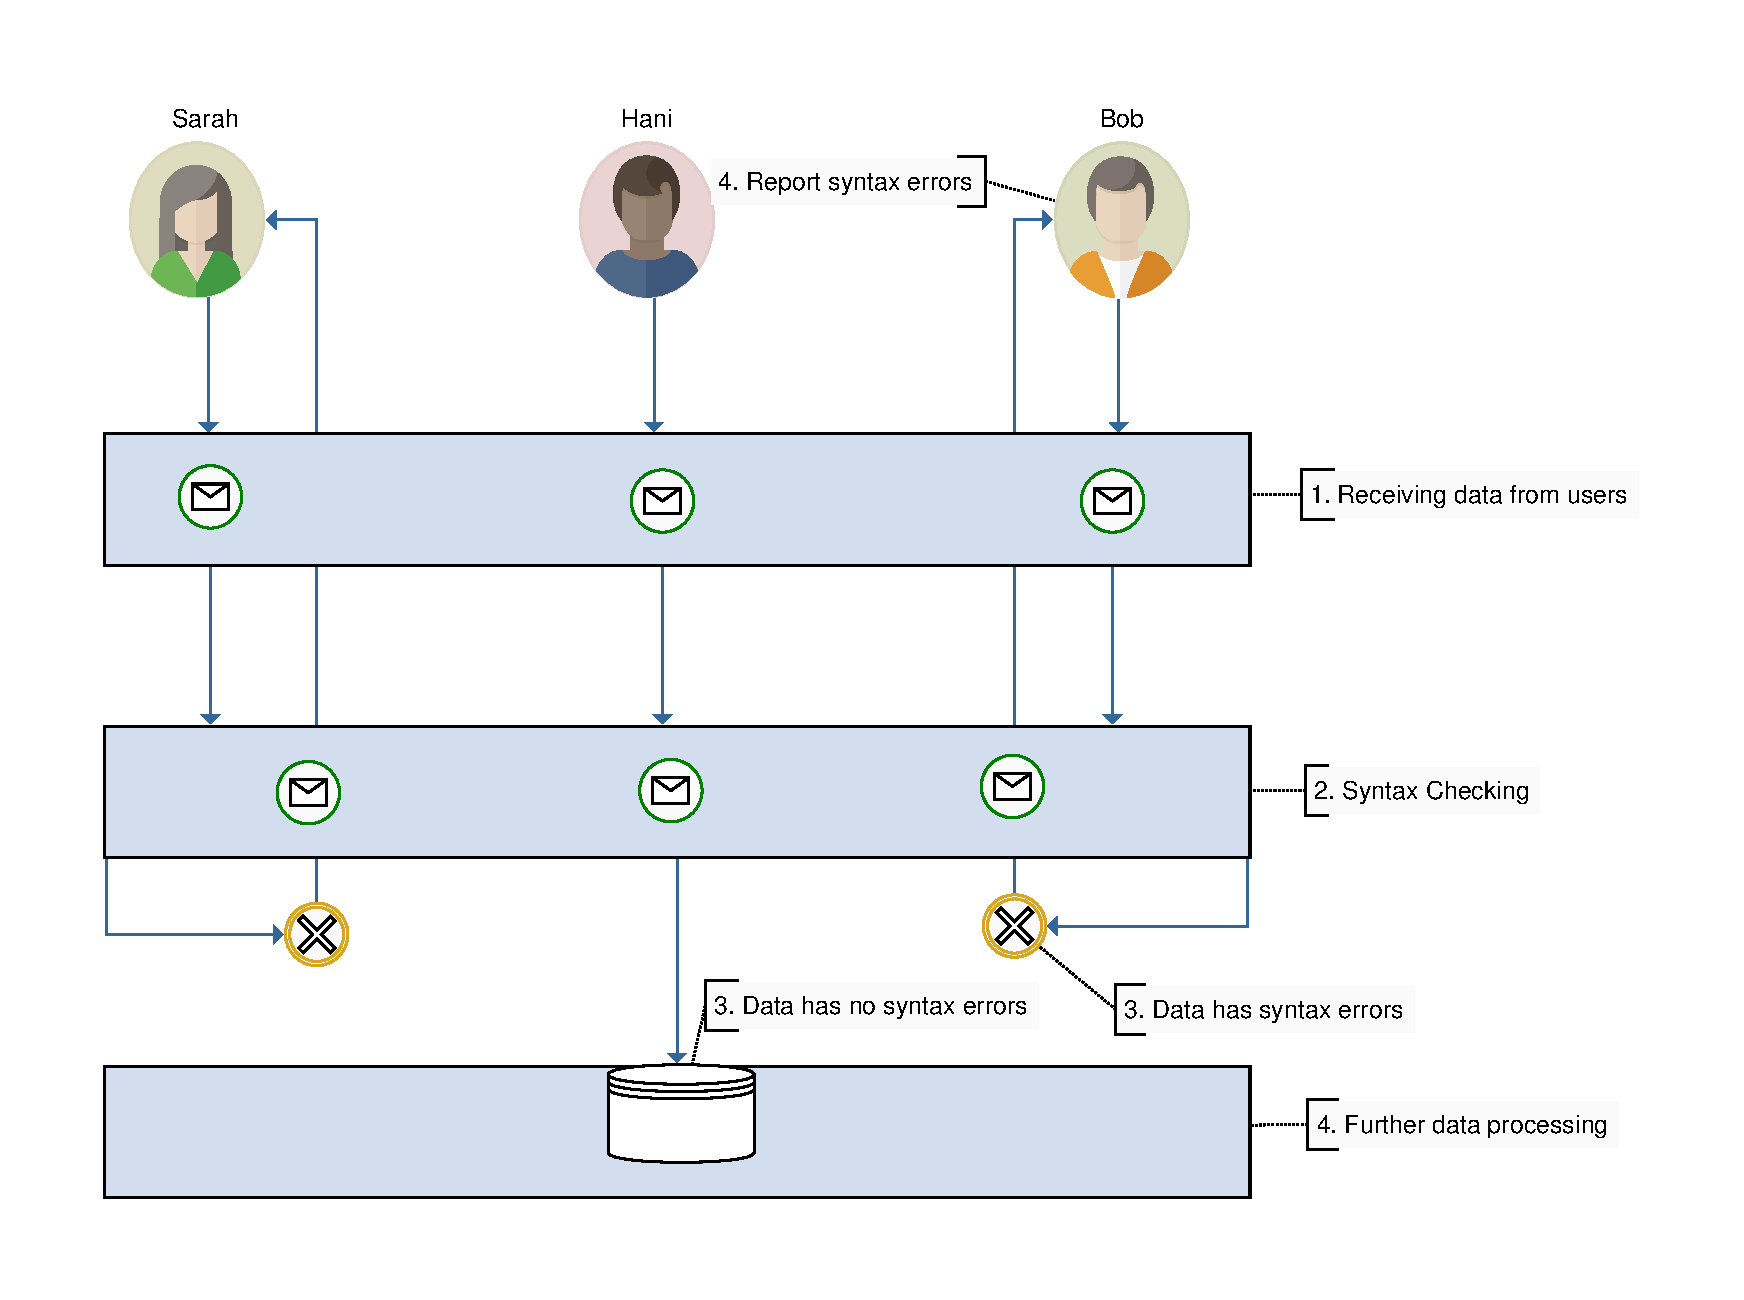
\includegraphics[width=0.9\textwidth]{images/motivation.pdf}
			\caption{\textbf{Motivation example.} Typical scenario where different ontology engineers send their ontology versions to the system for syntax validation before further data processing.
			Both Sarah and Bob have one syntax error or more, but they receive on error at time and they have to manually resolve it.
			On the other hand, the version of Hani passed with no syntax errors and goes to the next phase for further processing.}
			\label{Fig:Motivation}
	\end{figure}

%let's dig deep in demonstrating what is there in  {Figure \ref{Fig:Motivation}}, It is showing a flow of data from clients or users seeking further data processing. 3 persons are shown in this Figure, their names are Bob, Hani, and Sarah. All of them start with the first phase by sending their data to be syntactically checked. The parser starts checking if there are syntax errors of the input data, if such data passed with no syntax errors, it can be forwarded for further phases, i.e. for data processing, otherwise, the input data will send back to the user to correct the errors. {Figure \ref{Fig:Motivation}} clearly shows that Sarah and Bob have syntax errors in their input data,then, they got an error report, including details about the first detected error. In the meanwhile, Hani has received his data processed without getting such a report, since his input data has no syntax errors. 

%This study has been fostered by the former illustrated example to find a suitable solution to allow the parser to continue the whole input of RDF data checking against syntax error and to list them in an error report if any was found. Therefore, the proposed solution focuses on producing a software tool that can detect all syntax errors that can be detected in the input RDF data. 

%\section{Objectives}
\section{Problem Description and Challenges} 	
Ideally, ontology engineers should be able to retrieve and easily correct easily any existing error in their ontology version.
At the conceptual level, this thesis addresses the problem of comprehensive and simultaneous error detection and resolving for the RDF documents.
Therefore, the approach should assist ontology engineers on identifying syntactic issues and automatically fix them.
In addition, for any error that is not possible to automatically correct, a user-friendly and understandable message should be provided.

%Before reaching the proposed solution, different methods have been tired to reach the objective. 
Over the year several approaches have been presented for parsing RDF documents and finding syntactic errors.
%The main purpose was the continuation of parsing till the end of the file without stopping on the first syntax error detection  and storing details of the detected errors into a data structure, such as lists. 
Well-known tools, such as: Jena API \cite{McBride:2002:JSW:613357.613755}; RDF4J API \cite{RDF4J:Online}; and N3 Parser \cite{N3Parser:Online}, implemented as Java-based toolkits or as a Javascript-based parser, respectively, are used to process the N-Triple and Turtle serialization formats. 
Commonly, these tools utilize an exception handling mechanism to catch any potential syntax error and are able to recognize only one error at particular time.

We identified several challenges that should be tackled in order to achieve a comprehensive error coverage for RDF documents.
These challenges include: 1) finding the exact position in a given RDF document, where there error is occurring; 2) enabling the continuation of the parsing procedure after encountering of each error; 3) identifying multiple errors in the same line or subsequent statements; 4) automatic correction of a subset of errors; and 5) improving conflict resolution via user-friendly messages.
%Our task was to remove the text that contains the first detected syntax error from an input text (since those tools fail when the first syntax error is found), then, to supply the remaining text for further parsing. 
%Two methods were used: 1) cutting only the triple or the statement that contains the syntax error, 2) removing text before the found syntax error, including the statement of the error. 
%Both those methods were failed to offer a suitable solution for continuation of parsing after an error discovery, for the following reasons: 1) the difficulty of handling nearby syntax errors, such as errors in the same line or in subsequent statements follow each others, 2) the inexpressive and incomprehensible of error messages, especially, in the second tool, which complicates understanding the actual syntax error for further handling.    


%TODO need references.


\section {Contributions}
%In this study, the research work set out to syntactically check RDF data. 
The main contributions of the proposed approach are listed in the following:
\begin{enumerate}
	\item  {\bf Identifying of exiting syntax errors in RDF Documents:} is a major goal and contribution with the intention to investigate RDF Documents and search for potential syntax errors. 
	The proposed approach is powered by ANTLR framework \cite{ANTLR:Website:Online}, a powerful parser generator, with the objective of establishing an RDF parser that enables simultaneous listing of all discovered syntax errors. 
	The fundamental aspect of the approach is the injection of the grammar identification rules inside the parser. 
	Once, the parser detects a presence of so-called tokens in an RDF input matching one of the given grammar rules that represent a syntax error, it sends an error notification to the error listener component, where error lists are stored.
	\item {\bf Reporting syntax errors with user-friendly and expressive messages:} where either normal users or ontology engineers are assisted with meaningful error messages. 
	Following the principle from the ancient Greek philosopher, Socrates: “Understanding a question is half an answer”\cite{Socrates:quote:Online}, similarly, an understandable error message helps to recover from an error. 
	Our approach is based on both: the regular expression and grammar rules, where each rule represents either a sequence of correct syntax tokens or a sequence of incorrect ones. 
	In case of the latter, we encoded a predefined information about each error, hence, a customized error message can be formulated in an meaningful and convenient way and delivered on-the-fly to the error listener.  
	\item {\bf Automatic error recovery of a subset of syntax errors:}, which basically includes syntax errors similar to those in well-know programming languages, such as missing a dot, adding more than one dots, or missing semicolon. 
	A particular rule is designed to limit repeatable conflicts notifications while correcting errors and to control the eligibility of an error to be corrected. 
	The rule is check for the presence of a specific error in a predefined error correction list.
	It includes fundamentally common errors with information about the necessary actions for recovery procedure. 
	For instance, missing of a dot or a semicolon are common mistakes during editing of RDF Documents, and these errors can automatically corrected by our approach.
	However, there exists several errors, such as missing of a prefix declaration, that cannot be corrected since the details of that missing prefix are obscure and unknown.     
\end{enumerate}

\section {Thesis Structure}
The thesis is structured into seven chapters. 
%Until this spot, \textbf{Chapter \ref{ch:introduction}} was presented, titled with "Introduction". 
It starts with the \emph{Introduction}, where a general overview of the study, the motivation, the problem description and the challenges, as well as contributions are presented. 
The remainder of the thesis is organized as follows:
\begin{itemize}
	\item { \textbf{Chapter \ref{ch:preliminaries}:} describes the background knowledge which comprises relevant concepts and terminology required to understand the work that has been conducted in this thesis.}
	
	\item {\textbf{Chapter \ref{ch:related}:}} discusses the existing approaches from the state of the art related parsing of the RDF documents. 
		
	\item {\textbf{Chapter \ref{ch:approach}:}} presents the proposed approach along with its distinctive characteristics and important features. 
	
	\item {\textbf{Chapter \ref{ch:implementation}:}} demonstrates the actual implementation of our approach, including the architecture and its modules.
	
	\item {\textbf{Chapter \ref{ch:evaluation}:}} shows the evaluation part where the approach is tested in three different scenarios and the obtained results are discussed.

	\item {\textbf{Chapter \ref{ch:conclusions}:}} presents the conclusion of our work realized in this thesis and provides a number of potential future directions.
\end{itemize}








\chapter{Background}
\label{ch:preliminaries}

In this chapter, we outline the relevant terminologies and the theoretical  preliminaries that is essential for better understanding of this essay.
This chapter is sectioned into 3 parts.
Section \ref{sec:bck_rdf_model} describes essential concepts of RDF as a modeling language and its main serialization formats. 
In Section \ref{sec:bck_parser}, parsing techniques and methods to detect and recover syntax errors are discussed. Finally, Section \ref{sec:bck_ANTLR} presents an overview of ANTLR parser generator which is used to automatically generate the internal parser of RDF-Doctor.


\section{The Resource Definition Framework}
\label{sec:bck_rdf_model}

The "Semantic Web" \cite{W3C:SemanticWebTerm:Online} term  has appeared during the transformation process of web development from "Web of documents" to "Web of data", similar to those data found in databases. 
W3C defines it as "the Web of linked data". {Figure \ref{Fig:semanticWebStack}} describes the Semantic Web Stack, proposed by W3C. 
It can be seen that it contains several technologies to enable the users of creating their own data stores on web, building vocabularies, and enforcing processing rules on such data.   

Subsequently, in order to make data more and more machine-readable and interchangeable between various applications, RDF model \cite{W3C:RDF-Primer:Online} has been proposed.  To elaborate, RDF model plays a fundamental role of data exchange in the layered Semantic Web Stack and links the high-level semantic web tools with low-level ones, as exhibited in {Figure \ref{Fig:semanticWebStack}}. 
	\begin{figure}[ht]
	\begin{center}
	\setlength\belowcaptionskip{-7mm}
		\includegraphics[scale=0.5,angle=0]{images/semanticWebStack}
		\caption{\textbf{The Semantic web stack \cite{W3C:SemanticStack:Online}.} RDF Model links  high-level semantic web tools with low-level ones and works as a bridge to enable data exchange between various applications.}
		\label{Fig:semanticWebStack}
	\end{center}
\end{figure}
\par
Also, {Figure \ref{Fig:rdfModel}}(a) presents how data are engineered in RDF Model in triples. A triple is defined by 3 main components: a subject, a predicate, and an object. It has a common similarity of a basic structure of a simple sentence in a natural language which consists of a subject, a verb, and  an object. As the verb in natural languages shows a relation and a connection between the other two entities, in the same way in RDF Model, the predicate connects both subject and object in a certain property. 

\subsection{Simple Example of RDF Model}

To make it more clear, a simple example of RDF Modeling is giving in Figure \ref{Fig:rdfModel}(b). A fact to express that "German has the river Rhein", \textbf{Ex:Germany} is a subject, \textbf{Ex:hasRiver} is a predicate, and \textbf{"Rhein"} is an object. The first two terms are Uniform Resource Identifiers (URIs) where \textbf{Ex:} is a declared prefix label in RDF file to refer to an URI path and the following part \textbf{Germany} is an extension of the path. The last value \textbf{"Rhein"} is a literal or a string. What is given is a simple example of RDF Model to show its fundamental structure, but, in the meanwhile, more examples can be viewed at \cite{W3C:RDF-Primer:Online}.

\begin{figure}[ht]
	\begin{center}
		\includegraphics[scale=0.4,angle=0]{images/RDF-Model}
		\setlength\belowcaptionskip{-5mm}
		\caption{\textbf{ Structure of RDF with example.} A triple is a major component in RDF Model which has a form of Subject-Predicate-Object, as shown by (a), while an example of a triple is presented by (b).}
		\label{Fig:rdfModel}
	\end{center}
\end{figure}
RDF data can be represented in a couple of serialization formats, as was mentioned in Chapter \ref{ch:introduction} and since their syntax are used as use cases to be parsed with RDF-Doctor , In the next two subsections, Turtle and N-Triples are discussed. 


\subsection{Turtle Serialization}
 Terse RDF Triple Language (Turtle) \cite{W3C:Turtle:Online} is one of RDF serialization formats, it uses triples for data representation. A triple has Subject-Predicate-Object form, it  has a similarity with some of natural languages where a simple sentence consists of a subject, a verb, and an object. In order to understand the syntax of Turtle, some terms  relevant to its syntax are discussed in the following:

\begin{figure}[ht]
	\begin{center}
		\includegraphics[scale=0.8,angle=0]{images/TurtleStructure.png}
		\setlength\belowcaptionskip{-5mm}
		\caption{\textbf{ Structure of Turtle in example.} Multiple terms draw the syntax of Turtle, they are pointed with one or more matched samples.}
		\label{Fig:TurtleStructure}
	\end{center}
\end{figure}
\begin{itemize}
    \item \textbf{URI\footnote{https://tools.ietf.org/html/rfc3986
}:} it refers to a Uniform Resource Identifier, used to point to a web resource, not only a web page address, as a Uniform Resource Locator (URL) do. In two forms, it can represented by: 1) Absolute form (similar to URL in-between 2 brackets, in Figure \ref{Fig:TurtleStructure} lines 1 and 6, pointers show samples of absolute URIs); 2) Relative form or \textbf{Relative URI}, this form is used when a base URI is defined, in Figure \ref{Fig:TurtleStructure} line 5 shows a declaration of a base URI, then, line 12 shows two samples of relative URIs \textless Manager\textgreater and \textless manages\textgreater ; 3) Short form (referred as \textbf{Prefixed-Name} and discussed next).
  \item \textbf{Prefix:} a prefix declaration is a  short-cut way to replace absolute URIs with abbreviated ones. Essentially, it contains a \textbf{Prefix-Label} and \textbf{Prefix-URI}. Prefix samples are shown in the first four lines of Figure \ref{Fig:TurtleStructure}, starts with \textbf{@prefix} keyword, followed by a \textbf{Prefix-Label}, then a colon, next comes a URI or a \textbf{Prefix-URI}, and lastly, an end dot. 
        \item \textbf{Prefix-Name:} a short URI consists of a \textbf{Prefix-Label}, followed by a colon, then a resource name. A sample is pointed in Figure \ref{Fig:TurtleStructure} line 13.
        
        \item \textbf{Prefix-Label:} a short sequence of characters to get rid of  re-writing of a long absolute URI.
        \item \textbf{Prefix-URI:} an absolute URI are used in prefix declarations. 
        \item \textbf{Base:} a base declaration to define a base URI used inside a Turtle file. This could be also another short-cut way for URIs when they have a common path, then the last local part in URIs can be written inside 2 brackets.  
\item \textbf{Directive:} prefix and base declarations can be considered as directives, similar in somehow to those declarations of libraries in common programming languages.  
    \item \textbf{Blank Node:} an identifier for a temporal or unnamed resource \cite{journals:tkde:GutierrezHV07}, it starts with ":\_", then a sequence of characters (referred as BlankNode-Label). Figure \ref{Fig:TurtleStructure} line 13 shows a blank node in the position of Subject.  
    \item \textbf{Literal:} a string or a number (either numeric or boolean number). A string sample is exhibited in Figure \ref{Fig:TurtleStructure} line 9.
\end{itemize} 

The main players in Turtle syntax are prefixes and triples. Prefixes are used to make Turtle a user-friendly language and to reduce the redundancy of repeating absolute URI, subject, and subjects and predicates, if one subject and one predicate are together shared  more than one object. 

\begin{figure}[ht]
	\begin{center}
		\includegraphics[scale=0.4,angle=0]{images/TurtleandNtripleElements.png}
				\setlength\belowcaptionskip{-5mm}
		\caption{\textbf{ Elements of triple in Turtle and N-Triple serializations.} Triple consist of Subject, Predicate, and Object, Subject can be either URI or Blank Node (BN), Predicate is only URI, while Object can take URI, BN or Literal forms.}
		\label{Fig:TurtleandNtripleElements}
	\end{center}
\end{figure}


In order to understand the basic rules defined Turtle serialization, in the following text, those rules are outlined, however, more details and advanced rules are found at \cite{W3C:Turtle:Online}:
\begin{itemize}
    \item Each directive (a declaration of Prefix or Base) or triple ends  in a  dot.
    \item Figure \ref{Fig:TurtleandNtripleElements} shows which elements can replace the content of a triple as follows: \textbf{Subject} can be either a blank node, or URI, a \textbf{Predicate} is only URI, and an \textbf{Object} can be either an URI, a Literal or an blank node.
    \item When multiple \textbf{Objects} share the same \textbf{Subject} and \textbf{Predicate}, then comma symbols separate between those \textbf{Objects}, as demonstrated in Figure \ref{Fig:TurtleStructure} line 7, both \textbf{ex:animal} and \textbf{ex:mammal} objects with the same subject \textbf{ex:dog1} and the same predicate \textbf{a}  (a keyword substitutes the \textbf{rdf:type} URI) are separated by a comma.
     \item A semicolon separates combinations of a \textbf{Predicate} and an \textbf{Object} when these combinations share the same \textbf{Subject}. Both lines 8 and 9 of Figure \ref{Fig:TurtleStructure} shows this pattern where a combination of a predicate \textbf{rdf:type} and an object \textbf{ex:cat} and the other combination of a predicate \textbf{rdfs:label} and an object \textbf{"Lusi"@en}, share the same subject \textbf{ex:cat1}, then both combinations are separated by a semicolon.
      \item Prefix and Base declarations are generally written on the top of Turtle files or at least before using them in a Prefix-Name found in triples.
     \item Literals are strings or numbers. Strings have multiple forms: 1) a string in single line, written between 2 double or single quotes; 2) a string in multiple lines, starts with 3 double or single  quotes and ends in same number of quotes; 3) a string with a language tag, has the first 2 string forms, followed by \textbf{@}, next comes a language tag (a few sequence of characters to identify the language of the preceding string); 4) a string with a certain data-type, again has the first 2 string forms, followed by \textbf{\textasciicircum\textasciicircum}, then a data-type URI comes, \textbf{"Lusi"\textasciicircum\textasciicircum\textless http://www.w3.org/2001/XMLSchema\#string\textgreater} is a string sample of XML Schema data-type\footnote{https://www.w3.org/TR/xmlschema11-2/}. Numbers are numeric values, e.g., decimals, integers, and doubles or boolean values.
     \item Blank Node identifier refers to one resource must use the same identifier that refers the same resource in the whole Turtle file.   
     
     
\end{itemize} 

\subsection{N-Triple Serialization}
N-Triples \cite{W3C:Ntriples:Online} is the simplest  and a popular serialization format that forms RDF data in triples, however, it is hard to be read by users, since long absolute URIs are mostly used to represent \textbf{Subjects}, \textbf{Predicates}, and \textbf{Objects}. Figure \ref{Fig:NTriplesStructure} shows an N-Triple example where  only the following 3 elements serialize its content:  \textbf{Absolute URIs}; \textbf{Blank Nodes}; and \textbf{Literals}, they are same as those in Turtle serialization. 

Hence, N-Triple is considered as a subset of Turtle serialization. Additionally, the content of its \textbf{Subjects}, \textbf{Predicates}, and \textbf{Objects} are shown in Figure \ref{Fig:TurtleandNtripleElements}, again similar to Turtle, however, a type of absolute URIs is only used in N-Triple. So, N-Triples has no prefix or base declarations, repeats a subject even if it is shared with a combination of a predicate and an object, same also when multiple objects share the same subject and predicate. To end this, a general form of N-Triples can be reached,  consisting of a \textbf{Subject}, followed by a \textbf{Predicate},  next comes an \textbf{Object}, finally, ends in  \textbf{a dot}.   

\begin{figure}[ht]
	\begin{center}
		\includegraphics[scale=0.8,angle=0]{images/NTriplesStructure.png}
		\setlength\belowcaptionskip{-5mm}
		\caption{\textbf{ Structure of N-Triple in Example.} Main elements of N-Triples serialization are URIs, Blank Nodes, and Literals, samples of them are pointed. Local parts or resources of URIs are colored in black to make it a better human-readable, even it is not easy with those absolute URIs.}
		\label{Fig:NTriplesStructure}
	\end{center}
\end{figure}


\section{Parsing and Error Recovery}
\label{sec:bck_parser}
This subsection defines "Parsing" and "Grammar" terms, shows the role of the parser in the compiler, discusses types of parser developments, and finally, it lists the methodologies of error recovery in parsers. 
\subsection{Parsing and Grammar Definitions}
It is of great benefit to shed a light on parsing term to understand later the approach of this study. In \cite{parsingGuide2017}, Gabriele Tomassetti has defined \textbf{Parsing} by:{\it  \textbf{``The analysis of an input to organize the data according to the rule of a grammar''}}. It can be intelligibly recognized that parsing deals with some input data and tries to analyses it based on a given grammar. let's have a look on the definition of grammar based on  \cite{parsingGuide2017},as well. \textbf{Grammar} is 
{\it \textbf{``A formal grammar is a set of rules that describes syntactically a language''}}. In the definition, rules are the significant part of the grammar to define a syntax of a language.  
\subsection{Parser Role in Compilers}
The parser is an essential element in  compilers. {Figure \ref{Fig:parserPosition}} draws the role of the parser in a compiler. The first component "Lexical Analyzer" receives the input data, then produces tokens for  the "Parser" component. Parser constructs a parse tree based on its grammar rules and gets the next token until it consumes all the tokens. The parse tree as an output of the parser is delivered to the next phases of the compiler. If any errors are found, lexical errors can be generated by Lexical Analyzer and Parser is the producer of both syntax and semantic errors. 
%TODO{add the ref or change the image}

\begin{figure}[ht]
	\begin{center}	\setlength\belowcaptionskip{-5mm}
	\includegraphics[scale=0.55,angle=0]{images/ParserRole}
	\caption{\textbf{Role of Parser in compilers}. a parsing process in a compiler has 2 main elements: a Lexical analyzer and a parser, the former supplies tokens to the latter, once it has enough tokens to be parsed, it parse them, and asks the former to continue of the tokens supplement, the former generates lexical errors and the latter produces syntax ans semantic errors when parsing a source program, the parse tree is the output of the latter.}
		\label{Fig:parserPosition}
	\end{center}
\end{figure}
\subsection{Parser Developments}
In order to build a parser, there are two available options, either by starting  to code own parser  or getting an off-the-shelf automatic parser generator tool that automatically creates the parser source code from a grammar file. In the following, both approaches are outlined:

\textbf{1) Writing a parser source code from scratch:} it is to write own parser source code from A to Z, including the lexical analyzer and the parser classes. On the one hand, this way gives more flexibility in handling several issues, triggered when dealing with certain token patterns, such as special characters and escape sequences. On the other hand, it consumes much time and requires a large amounts of  effort.

\textbf{2) Generating a parser source code using automatic parser generators:} a parser generator outputs the desired parser source code. Predominately, such tools can be used to do a specific parsing task, but again, a grammar identifying the  demand syntax is required as an input for those tools. To elaborate, the competitive advantage here is the less needed time and effort to build a parser, However, the flexibility is reduced to what features and classes provided by those tools, otherwise, such flexibility can be  optimized by adding new classes and modules to more features, for example to parse a large file, frequently, an "full memory space" error is fired, by adding a class that divides the large file into chunks to be sequentially parsed, can solved this issue and add such new feature.  

\subsection{Error Recovery Methodologies in Parsers}
In parsers, the error recovery techniques specify the parser behavior, once an error is detected.  Aho et al \cite{Aho:2006}, the researchers in the compiler field    have outlined such techniques as follows:
\begin{itemize}
	\item \textbf{Panic-Mode Recovery}: once an error has been discovered, the parser ignores and skips next input symbols, one by one till a recognized set of tokens is detected. In spite of its discarding of huge number of input symbols without checking them for further error detection, it is considered a simple parsing mode and do not fall in an infinite loop while other modes may do.
	\item \textbf{Phrase-Level Recovery}: to continue the parsing process, the parser performs local correction. A typical local correction in RDF data, for example, is to insert a missing dot or delete extraneous dots.
	\item \textbf{Error Productions}: by expecting  common and well-known errors, production rules can be inserted into the grammar. Then, the generated parser is well-informed about such errors. Error detection and error recovery can be easily done in this case where error details are in our hand, such as the error location, the exact type of error, etc. Equally important a customized and meaningful error message for the identified error can be provided as well. 
	\item \textbf{Global Correction}: conventionally, the parser tries to reduce as much as possible number of change operations (such as, insertion, deletion and modification operations), when dealing with an incorrect input token to reduce globally total cost of error correction. To make it more clear, let's assume an incorrect input statement X is giving in grammar G, the parser constructs a closest error-free parse tree of statement Y to replace statement X, such that the changes are small as possible. 
\end{itemize}


\section{ANTLR Parser Generator}
The parser module in RDF-Doctor was automatically built with a help of ANTLR Parser Generator based on our grammar as an input, as well as,  the ANTLR library is used as a plug-in. In the following text, a short overview of ANTLR and its generation process of a parser are discussed.   
\label{sec:bck_ANTLR}

\subsection{ANTLR in a Nutshell }
ANTLR is a handy tool and easy to use for the purpose of generating a specific domain language parser. It is a parser generator to do an automatic generation of a source code of a parser with less time and effort. The core requirement of ANTLR is to define a grammar of a desired language syntax . The grammar contains desired language rules  drawing the syntax and the semantic of such  language which the parser is built for. 
\subsection{ ANTLR as a Parser Generator }
 As was previously discussed, the compiler has two main subsystems relevant to this study: a lexical analyzer (called also lexer) and a parser. Both lexer and parser are needed to have their rules defined in the grammar file. Lexer rules are those rules which define the terminals, whereas parser rules determine the non-terminals. Another essential point that is the process of parser creation  demonstrated in {Figure \ref{Fig:ANTLR} where the parser program is generated with the help of ANTLR framework. In more details, this parsing process \cite{ANTLR:Tool:Online} is followed, starting from the needed grammar to build the parser, ending with the output of the parse tree at the end of parsing :

\begin{figure}[ht]
	\begin{center}
		\includegraphics[scale=0.52]{images/ANTLR.pdf}
				\setlength\belowcaptionskip{-5mm}
		\caption{\textbf{Parsing process based on ANTLR parser generator\cite{ANTLR:Tool:Online}.} ANTLR parser generator receives the grammar file to generate the classes of the lexer and the parser, when the input text is submitted, the generated classes with using of ANTLR library start the parsing process to generate the parse tree.}
		\label{Fig:ANTLR}
	\end{center}
\end{figure}


\begin{enumerate}
		
		\item  {\bf Writing a grammar file:} ordinarily, a grammar called a parsing expression grammar (PEG) is required to build a parser. ANTLR needs a context-free grammar, crafted with the Extended Backus-Naur Form (EBNF). EBNF consists of a sequence of rules. These rules describe the syntax and the semantic of an input which needs to be parsed. Both terminals or non-terminals are types of rule heads. On the one hand, terminals are leaf elements where they have no grammatical structure, e.g., words or numbers. On the other hand, non-terminals have a definite grammatical structure and name, e.g., triples or prefixes. 

		\item {\bf Generation of recognizer target\_based classes by ANTLR:} a significant feature of ANTLR is its capability of generated the auto-generated parser source code for  a variety of the programming languages like \cite{ANTLR:Website:Online}: Java, C\#, Python (2 and 3), JavaScript, Go, C++, and Swift.
		\item {\bf Feeding an input file for parsing:} as an input, ANTLR can parse text documents without additional libraries. Users send their input files for parsing where the parsing process will be achieved based on the crafted grammar in the first step.
		\item {\bf Parsing procedure:} {Figure \ref{Fig:ANTLR} } shows this step as  a phase of cooking . In this step, all materials and ingredients are available. The materials are: 1) the auto-generated parser, and 2) the ANTLR library. The ingredients are one or more text files to be parsed. 
		\item {\bf Delivering of a final report and parse tree as an output:} now, the cake is ready for eating, an output of this process is given to the user containing of a parse tree and a report of collected errors.
	\end{enumerate}












\chapter{Related Work}
\label{ch:related}


%In this chapter, we focus on previous work that is related to the problem stated in \nameref{ch:introduction}. 
This section reviews the state-of-art of research works in the field of RDF syntax parsing and checking.

\section{RDF Parsing and Syntax Checking Approaches}
In order to validate RDF data as an input, either by inserting a URL where it exists or by uploading a file, almost the available tools and applications that we could find, can only offer the first detected syntax error while consecutively parsing that input from its start point to its end point. Moreover, semantic developers and engineers are struggling whilst debugging their RDF data and they necessarily need alternative tools that could be more helpful. To the best of our knowledge, there is no comparable prior work regarding fault-tolerant parsing and syntax checking of the diverse RDF serialization formats expect one that can only work for an RDF/XML format. Hence, a tool that can prominently list of all errors included in the RDF data is desired.
\subsection{RDF/XML Parsing Tools}

 Despite the existence of  several theoretical models and practical tools that have been invented in the same field, we can hardly find a research that cares of finding more than one syntax error inside RDF data. Moreover, during our journey of searching the existing tools that provide such a service, the W3C RDF validation tool \cite{W3C:Validation:Online} was firstly checked, it is an web tool, available online for the purpose of parsing and validating RDF/XML codes. It uses the ARP parser of Jena \cite{McBride:2002:JSW:613357.613755} as its core, however, it fails in detection of multiple syntax errors and the first error in order was only released as shown by Figure \ref{Fig:errorW3RDFValidator}.
 
 In 2000, a Validating RDF Parser (VRP) \cite{karsten:Thesis:2000} was developed by K. Tolle in his thesis, it is a Java-base parsing tool, features semantically and syntactically checking of an RDF/XML format. Nevertheless, the validation service provided by VRP is limited to parse only a format type of RDF/XML and does not support other RDF serialization formats, such as N3, N-Triple, and Turtle. Figure \ref{Fig:VRPErrorResult} shows that VRP can list more than one error or first detected error. An RDF/XML file with the same text applied in Figure \ref{Fig:errorW3RDFValidator}, included 2 syntax errors was used as an input to test VRP. As a result, 4 error messages were given, 2 of them are very related to the injected errors and significantly meaningful to correct them, whereas the other 2 messages are with no benefits and have no relation to them, they are false positives. Differently, in this work, a general approach that can work for all RDF serialization formats is planned, however as use cases, Turtle and N-Triple formats have been considered  while developing RDF-Doctor to prove our assumption. 
 
 \begin{figure}[ht]
		\begin{center}
			\setlength\belowcaptionskip{-7mm}
			\includegraphics[scale=0.8,angle=0]{images/errorW3RDFValidator.png}
			\caption{\textbf{Validation results of the W3C RDF validation tool \cite{W3C:Validation:Online} after parsing an RDF/XML text, included two syntax errors.} The original RDF/XML document has two syntax errors since "rdf1" and "dc12" have no prefix declarations, but the results under "Fatal Error Messages"  show only the first found error and neglects the other.}
			\label{Fig:errorW3RDFValidator}
		\end{center}
	\end{figure}
\subsection{Several Serialization Formats  Parsing Tools}

\par Next, the existing tools that validate more than one  RDF serialization formats rather than only parsing of RDF/XML format were checked. We have started with Jena RDF toolkit \cite{McBride:2002:JSW:613357.613755} which offers validation service based on the ARP parser. It can  be also used as a standalone program using a command-line  or as an API, integrated within another application. Considering its powerful capability of validating numerous RDF serialization formats, including RDF/XML, again, the first error is only reported.
 \begin{figure}[ht]
		\begin{center}
			\setlength\belowcaptionskip{-10mm}
			\includegraphics[scale=0.7,angle=0]{images/VRPErrorResult.png}
			\caption{\textbf{Validation results of Validating RDF Parser (VRP) \cite{karsten:Thesis:2000} after parsing an RDF/XML file, included two syntax errors.} 4 error messages are shown, 2 of them are meaningful, hence, they help in resolving the 2 detected errors, the other 2 messages have no meaning.}
			\label{Fig:VRPErrorResult}
		\end{center}
	\end{figure}
\subsection{Classification of parsing approaches based on its core}

Some of the tools validating RDF formats use the following core tools or methods as a significant part of their implementations. which tool  uses which core component is discussed in the following : \begin{itemize}[noitemsep] 
	\item \textbf{ARP-parser-dependable approach :} both W3C RDF validation tool \cite{W3C:Validation:Online} and RDF Validator and Converter \cite{Mybluemix:Validation:Online} use the ARP parser of Jena framework \cite{McBride:2002:JSW:613357.613755}. However, the latter focuses more on triple-based serialization formats, validating them and converting from one format to another, whereas the former validates only RDF/XML format. 
	\item \textbf{N3-parser-dependable approach :} N3 parser \cite{N3Parser:Online} is a JavaScript\_based syntax validator, mainly, developed for checking the syntax of Turtle and N-Triple formats. The online version of IDLab Turtle Validator \cite{IDLab:Validation:Online} uses N3 parser and it is integrated as a NodeJS plug-in. As well, the same approach was used to build a turtle editor with syntax validation in \cite{petersenturtleeditor}. However, this approach is slow when parsing and its behaviour is unpredictable when dealing with large files. 
	\item \textbf{Shape expressions approach:} in \cite{prud2014shape} a turtle parser was developed based on shape expressions. Shape expressions validates RDF through declaring of constraints on the RDF data, if the declared constraints are violated, then RDF data is invalid, otherwise, it is valid. Furthermore, Shape expressions describes the RDF graph based on regular expressions. 
\end{itemize} 

The previous three approaches failed to list more than the first found error. Another essential point has been learned is to avoid JavaScript\_based development of the new tool and the alternative is to use Java\_based application, similar to the ARP-parser discussed in the first approach. Empirically, developing using java can improve the performance of the purposed tool, especially when  validating large RDF data files.

\section{Types of Error Messages in Approaches}
Releasing user-friendly and meaningful error messages is of a great benefit to help the user to identify and correct the errors. 
\begin{itemize}
    \item \textbf{Non-expressive and meaningless error messages:} the parsing tools under the Shape expressions approach show less expressive  and unfriendly error messages.
    \item \textbf{Expressive error and meaningful  messages:} the parsing tools of ARP-parser-dependable approach and N3-parser-dependable approach  are presenting more expressive and user-friendly error messages which can provide the syntax error and its location in a proper way. 
    
\end{itemize}

\section{Error Recovery Approach}
Automatic error recovery or correction will be valuable to resolve from common syntax errors. For example, lots of programming languages need a semicolon at the end of the line. There are also few tools which can correct such errors without the involvement of the programmer. In the same way it will be useful to have this option of automatic correction after parsing of various serialization formats of RDF. Further, while surveying the existing RDF parsing tools, a tool proposed or provided such a feature was not found. RDF-Doctor will be equipped with this feature to correct these errors.   

\section{Summary}
To end this chapter, after describing the actual issue, reviewing the  state-of-art of research works, related to the same spot with pointing out  the different approaches of RDF parsing and syntax checking, different types of error messages , and finally the approach of automatic error correction. The outcome of this study is the RDF-Doctor. It is a parser that is generated with the help of the ANTLR parser generator. Additionally, It is a Java\_based application to parse N-Triple and Turtle serialization formats; show a meaningful error messages; as well as, automatically recover from common syntax errors.    











\chapter{Approach}
\label{ch:approach}
%As has been discussed in Chapter \ref{ch:related}, there is a need for a tool which can detect all the encountered syntax errors in RDF documents to ensure their quality and to make RDF diagnostics easy for users instead of showing only the first detected syntax error, struggling them in finding the other syntax errors if exist. 
In this chapter, we present RDF-Doctor, an approach towards realization of a comprehensive parser for syntax validation and recovery.
RDF-Doctor is able to identify more than one syntax error at the same time, and provide meaningful messages.
%order to fill this need, this study was held to propose a proper solution. 
Next, main components of RDF-Doctor are discussed in detail as well as possibilities of integration serialization formats, such as Turtle and N-Triple.


\section{Overview of RDF-Doctor Approach}

This section covers the core component of the approach, then discusses the main processing steps, and ends with elaborating the categories of RDF syntax errors to ease the road to the appropriate solution. 

\subsection{ANTLR: The Core Component}

As a core component inside RDF-Doctor is the ANTLR framework, it is used to automatically generate a parser based our developed grammar, including predefined error production rules to match sequences of tokens that contains RDF syntax errors.
%In order to find a parser which can accept the error production rules in its grammar, our choice was to use ANTLR framework to automatically generate the required parser.
%Equally important lots of handy features in ANTLR motivate its usage in the proposed solution to generate the internal parser, and also as an imported library for compiling and  running  of RDF-Doctor. 
The ANTLR framework has several important features: 1) a given grammar can equip with error production rules and when a couple of tokens match such rules, the parser will fire an error notification; 2) it uses a parse tree to parse input tokens and the view of this parse tree can be delivered as one of the outputs to the user at the end of parsing process; and 3)it supports the auto-generation of parsers in different programming languages.
%which is an one-to-many added value, where one grammar file can automatically generate of the programming languages.

%\begin{itemize}
% \item \textbf {Input}: It is the role of the user to provide an RDF file with certain options, such as 1) enabling/disabling of the error correction; 2) showing an error report of JSON\footnote{https://www.json.org/} or text format; and 3) concealing/showing up the parse tree.


%\item \textbf{Processing}: starts with preparing the input to be parsed in the following workflow: 1)it reads the input; 2) splits it into smaller pieces if needed; 3) parses the input for each slice (if many); and 4) corrects a subset of detected syntax errors. 
%This phase utilizes the parser built based on a predefined grammar.
%it requires ANTLR library for parsing, and some options from the user to activate/deactive some features of the solution.   
%\item \textbf{Output}: provides the reports after processing phase, %including 1) an error report to announce the detected syntax errors; 2) a correction report which lists the recovered syntax errors; and 3) an output file after healing some of the detected syntax errors\todo{It is not clear what is the point number 3}; and 4) a frame contains the parse tree. 
%Both, the correction report and the output file require to be enabled in order to be generated. 
%\end{itemize}


\subsection{Main Processing Steps}

\begin{figure}
	\centering
	  	\includegraphics[width=1\textwidth]{images/Approach.png}
		\caption{\textbf{RDF-Doctor workflow.} The user writes or edits his own RDF file, then sends it to RDF-Doctor for parsing.
		Next, RDF-Doctor can divide the input in multiple chucks, in case of a large input or use the same input file. 
		Each input chunk or file is parsed to detect any syntax errors if exist, then it recovers subset of detected errors, if the automatic error recovery feature is enabled by the user. 
		Finally, RDF-Doctor outputs a parse tree, a correction report, an error report, and an output file, including RDF file after error recovery.}
		\label{Fig:Approach}  
\end{figure}

The workflow of RDF-Doctor illustrated in Figure \ref{Fig:Approach} and its architecture depicted in Figure \ref{Fig:Architecture} are discussed in the significant steps of RDF-Doctor in the following:
%shows the technique used to handle an RDF text, including a couple of  syntax errors. 
%In the following, the main milestones of this approach are explained in 4 sequential steps:

 \begin{enumerate}[label=(\alph*)]
\item \textbf{Reading RDF files}: An ordinary RDF file is submitted to RDF-Doctor, this is the Input phase, as described in Figure~\ref{Fig:Approach} (a).
Initially, Processing components in Figure \ref{Fig:Architecture} read the submitted file. In case that file is too large (more than 1 million triples), then it is segmented into two or more chunks based on the number of triples. 
Each chunk is parsed and processed separately from others in this step.
%%%%%%%%%%%%%%%%%%%%
Moreover, certain options can be selected by the user before submitting of the file, such as 1) enabling/disabling of the automatic error correction; 2) showing an error report in either  JSON\footnote{https://www.json.org/} or text format; and 3) concealing/showing up the parse tree diagram at the end of parsing process.
%%%%%%%%%%%%%%%%%%%%
%{Figure \ref{Fig:Approach}}(a) simulates the actual work of this step where a submission of an RDF file with syntax errors is assumed. 
\item \textbf{Detecting of syntax errors}: Parsing is the 3\textsuperscript{th} step in  the Process phase in Figure \ref{Fig:Architecture}, in which the parser has predefined rules for syntax errors,  %(these rules are titled with error production rules, presented in Error Recovery Methodologies in Chapter \ref{ch:preliminaries}), 
\begin{figure}[ht]
	\begin{center}
		\includegraphics[scale=0.5]{images/architecture.pdf}
	\setlength\belowcaptionskip{-5mm}
		\setlength\abovecaptionskip{-2mm}		\caption{\textbf{RDF-Doctor architecture.} It consists of Input, Processing, and Output phases. 
		In the Input phase, users send their RDF data. The Processing phase reads these data, splits them in case of large volumes, then continues parsing and recovery of certain errors.
		In this phase a user action is action is required to enable/disable the error recovery.
	    Finally, Output phase presents reports for error detection and recovered error as well as the parse tree.}
		\label{Fig:Architecture}
	\end{center}
\end{figure}
once a rule is matched with a sequence of input tokens, it raises a flag to the error listener API which later is listed in the final error report. 
Reading of input tokens continues till the end of the file while searching for any match in order to identify potential syntax errors. 
In {Figure \ref{Fig:Approach}}(b) lines surrounded with \emph{red color} depict the detected lines which contain syntax errors.
%%%%%%%%%%%%%%%%%%%%%%%
%%%%%%%%%%%%%%%%%%%%%%%
To have a deep thought on the internal works of the parser to detect syntax errors using a parse tree, Figure \ref{Fig:approachParseTree} shows how each sub-tree of the root node (acts as the starting rule) is a rule containing either a correct syntax or an incorrect one, each rule is represented by a sub-tree having empty or one and more non-terminals (considered as rules in the grammar) and one and more terminals (they are lexical forms of input tokens). A sub-tree produces an syntax errors, if all of its terminals are formed one of error production rules, shown in \emph{red color} in Figure \ref{Fig:approachParseTree}. Hence both sub-trees 2\textsuperscript{nd}, and 4\textsuperscript{th} from left are rules with a sequence of tokens producing syntax errors.  Meanwhile other sub-tree 1\textsuperscript{st}, and 3\textsuperscript{rd}, and 5\textsuperscript{th} with terminals in \emph{green color}  are including  correct syntactic  forms.


\item \textbf {Healing a subset of encountered syntax errors}:%%%%%%%%%%%%%%%%%%%%
 { Figure} \ref{Fig:Architecture} shows this feature as the  4\textsuperscript{th} of processing components. %%%%%%%%%%%%%%%%%%%%
Firstly, it needs to be manually activated by the user, by default, it is disabled. Secondly, the method of syntax error recovery currently focuses on a certain type of errors which has only one predefined solution to correct them. Examples of such errors are  missing of a \emph{dot at the end of a triple}, missing a \emph{semi-colon after multiple predicates sharing same subject}, or missing a \emph{comma after multiple objects having same subject and predicate}. Lines surrounded with green color in {Figure \ref{Fig:Approach}}(c) represents some of healed lines from error at the end of the correction phase. 

\item\textbf {Producing of the output}: The output phase, demonstrated in Figure \ref{Fig:Architecture}, assumed the activation of automatic correction feature by the user as well as {Figure \ref{Fig:Approach}}(d) describes how the output file looks like at the end of this phase.    It shows lines containing errors are already recovered, whereas other lines still are unhealed. Commonly, errors that cannot be recovered by RDF-Doctor without user intervention, are those errors which can have several solutions, for example, a literal with multiple language tags like "me"@en@de which shows a string with two language tags and since the solution would be an omission of one of them but the intention of the user is unknown in this sense. In addition, there exist errors with undefined or unknown recovery solution, for example, missing of a user-defined prefix declaration for a certain local namespace which cannot be guessed since it is only known by the user himself. 
\end{enumerate} 
\begin{figure}
	\centering
	  	\includegraphics[width=.8\textwidth]{images/approachParseTree.png}
		\caption{\textbf{Detection of syntax errors while traversing the parse tree.} 
		Root node is the head of first rule in the grammar and the head of the parse tree.
		All the children of the root are either non-terminal nodes represented by "NT" followed by an number or  terminal ones shown by "T" succeeded by a number. 
		A syntax error can be detected on a non-terminal node when all of its terminals represent a sequence of tokens that is a statement including a syntax error. Red terminals represent error-inclusive statements and green ones for error-free statements.}
		\label{Fig:approachParseTree}  
\end{figure}


To functionally represent the approach of this study, Algorithm \ref{alg:algorithm-main} was engineered. 
It shows the abstract behaviour of RDF-Doctor where \textbf{syntaxRules} variable combines both correct syntax rules and incorrect ones. 
A \textbf{while loop} carries on until reaching the current end of file or chunk, if a large file is separated into several chunks. 
The \textbf{ruleToBeMatched} variable incloses one rule of either correct or incorrect production rules, formed by the supplied tokens. While the variable \textbf{currentTokens} stores a sequence of current supplied tokens to check to which rule, it belongs.  

Since the crucial step is to find encountered syntax errors, for that reason \textbf{ruleToBeMatched} is evaluated to check if its content are matched any of \textbf{incorrectSyntaxRules}, if this the case, then the content of \textbf{currentTokens} is considered as a syntax error and the parser sends an error notification to any subscribed error listener API, in order to further process of the collected errors. 

\begin{algorithm}[] 
 \caption{The pseudo-code of RDF-Doctor}
 \label{alg:algorithm-main}
 \KwData{inputText, correctSyntaxRules, incorrectSyntaxRules, CorrectionIsSelected}
 \KwResult{foundSyntaxErrors and recoveredSyntaxErrors}
% S = subject(M)\;
foundSyntaxErrors = [ ];\\
recoveredSyntaxErrors = [ ];\\
$syntaxRules \leftarrow correctSyntaxRules + incorrectSyntaxRules;$\\
		\While{token in inputText \&\& $inputText \neq EOF$}{
		currentTokens += token;\\
ruleToBeMatched += lex(token);\\
		\uIf{ syntaxRules contains ruleToBeMatched}{
		\uIf{ incorrectSyntaxRules contains ruleToBeMatched}{
		 foundSyntaxErrors.push(currentTokens);\\
		\uIf{ CorrectionIsSelected}{
		\uIf{ canErrorRecovered(ruleToBeMatched)}{
		  \uIf{recoverSyntaxError(currentTokens)}{
		  recoveredSyntaxErrors.push(currentTokens);\\
		  foundSyntaxErrors.pop(currentTokens);\\

		  }
		}
		}
		}
		 $currentTokens \leftarrow ""$  \\
		 $ruleToBeMatched \leftarrow ""$  \\
		 $token \leftarrow ""$  	\\	
		}
}
return foundSyntaxErrors , recoveredSyntaxErrors
\end{algorithm}

The automatic correction of errors is a feature that can be activated as an additional option when running RDF-Doctor. 
In case the user selects to enable it, then the \emph{Error Correction Module} will traverse all list of detected syntax errors and based on the error message, it can identify if the error can be unquestionably corrected or needs a user intervention. 
At the end of the correction phase, a report of the corrected errors will be delivered to the user. 

\section{Categories of RDF Syntax Errors}

In this approach, Turtle and N-Triples RDF serializations are used as the use case syntaxes. 
Hence, Turtle is a special case of N-Triples, for this reason, the grammar of RDF-Doctor was created based on Turtle serialization. 
Furthermore, since the significant part in this study is the ability to identify syntax errors, the expected syntax errors need to be known in advance, in order to be injected in the grammar. 
A suite of Turtle syntax errors are presented in ~\cite{TurtleTests:Online} plays an important role in syntax errors declaration. It contains several files in Turtle with an objective of showing both correct and incorrect syntaxes. Additionally, a filename in~\cite{TurtleTests:Online}, i.e., if it contains the word "Bad", means that it contains an incorrect syntax, which can be syntactically engineered in our grammar.

 \begin{table*}[tbp]
 	\centering
\includegraphics[width=5.5in]{images/TrimmedBigTable.pdf}
		\setlength\abovecaptionskip{-10mm}
	\caption{\textbf{Categories of a subset of syntax errors of N-Triple and Turtle serializations}.
	This table is a part of Table \ref{tab:syntaxErrorCate} which shows one sample of each category, the serial numbers take the same order of rows in the referred table. 
	Position represents a term related to Turtle and N-Triple serializations where the actual syntax error is located.}
	\label{tab:trimmedTable}
\end{table*}


In table \ref{tab:trimmedTable}, we have categorized types of syntax errors into multiple categories. This categories are taking from the filenames in~\cite{TurtleTests:Online} with some modification to make meaningful. The table shows each category with one error sample and an error position where the actual syntax error is located. Indeed, this helps much in designing of the grammar rules and also to identify which of them can be automatically corrected. Details including more samples of these categories are provided in Table \ref{tab:syntaxErrorCate}.     

\chapter{Implementation}
\label{ch:implementation}


In this chapter, details of the implementation practical part of the study is discussed. The architecture, modules, development tools, installation, and configurations of such part are the main role of this chapter.    
\section {Architecture}

	\begin{figure}[ht]
	\begin{center}
		\includegraphics[scale=0.5,angle=0]{images/Architecture}
		\caption{The proposed solution architecture}
		\label{Fig:Architecture}
	\end{center}
\end{figure}
\section {Modules} 
After briefing the proposed solution architecture, It is the time to cover it in more details by shedding light onto those modules which represent the pillars of such solution. The following text discusses 3 main modules of this solution:  
\section{Real-World Use Cases}
In this section, some of use cases tackled in this study to detect syntax errors in RDF input and  the method of error correction of some of those detected syntax error will be exposed. As a start, let's begin with a Turtle example which has no syntax errors, then some syntax errors can be included, then the process of handling them can explained. 
	\vspace{5mm} %5mm vertical space

Listing \ref{lst:turtleExample} shows a Turtle example without syntax errors. First 4 lines are directives or prefixes declaration. 

\begin{lstlisting}[label=lst:turtleExample, numbers=left, caption={RDF example in Turtle serialization format}]
<@\textcolor{blue}{@prefix}@>  <@\textcolor{red}{rdf}@>: <@\textcolor{orange}{<http://www.w3.org/1999/02/22-rdf-syntax-ns#>}@> .
<@\textcolor{blue}{@prefix}@>  <@\textcolor{red}{rdfs}@>:  <@\textcolor{orange}{<http://www.w3.org/2000/01/rdf-schema#>}@> .
<@\textcolor{blue}{@prefix}@>  <@\textcolor{red}{ex}@>:  <@\textcolor{orange}{<http://example.org/>}@> .
<@\textcolor{blue}{@prefix}@>  <@\textcolor{red}{zoo}@>:   <@\textcolor{orange}{<http://example.org/zoo/> }@> .
<@\textcolor{red}{ex}@>:dog1  <@\textcolor{red}{rdf}@>:type  <@\textcolor{red}{ex}@>:animal .
<@\textcolor{red}{ex}@>:cat1  <@\textcolor{red}{rdf}@>:type  <@\textcolor{red}{ex}@>:cat ;
         <@\textcolor{red}{rdfs}@>:label   <@\textcolor{green}{"Lusi"@en}@> .
<@\textcolor{red}{ex}@>:cat  <@\textcolor{red}{rdfs}@>:subClassOf  <@\textcolor{red}{ex}@>:animal .
<@\textcolor{red}{zoo}@>:host  <@\textcolor{red}{rdfs}@>:range  <@\textcolor{red}{ex}@>:animal .
<@\textcolor{red}{ex}@>:zoo1  <@\textcolor{red}{zoo}@>:host  <@\textcolor{red}{ex}@>:cat2 .
\end{lstlisting}











\chapter{Evaluation}
\label{ch:evaluation}
\newpage

\section{Experiments and Results}
To evaluate the proposed solution, firstly, it was tested against standard test cases, secondly, it was compared against XTurtle framework, lastly, it was validate with arbitrary large RDF files. This chapter discusses all of such details in the following text. 


\subsection{Testing with RDF SuiteTest}
The evaluation phase finds its starting point at \citealp{TurtleTests:Online} where Test Suite files of Turtle serialization are found. Any new parser (focused on the same RDF serialization) can its proficiency be validated against these files. 

In  \citealp{TurtleTests:Online}      
\subsection{Comparing the Proposed solution and Xturtle}
\subsection{Validation against arbitrary large RDF files }

\section{Accuracy}

\section{Scalability}









\chapter{Conclusion and Future Work}
\label{ch:conclusions}
\section{Conclusion}
This chapter concludes this study. Mainly, the focus was to detect all syntax errors in RDF input .  

\section{ Future Work}
The semantic web is rapidly developed, by introducing new tools, apps, plugins, can be of different programming language. As well, there are several RDF serialization  formats have same shortage of fault-tolerant parser. Since it a very wide and an open research field, a couple of ideas come to our mind which can be our next step in the future. 
\begin{itemize}
    \item Introducing parsers for mostly used programming languages. 
    \item Providing parsers to support the different RDF serialization formats.
    \item Developing to advanced parsers which parsing process in distributed manner.
\end{itemize}



%% ----------------------------------------------------------------
\clearpage
%------------------------------------------------------------------------------
\label{Bibliography}
\bibliographystyle{unsrtnat}  % Use the "unsrtnat" BibTeX style for formatting the Bibliography\bibliographystyle{plain}
\nocite{*}
\bibliography{literature}  % The references (bibliography) information are stored in the file named "Bibliography.bib"
\appendix
\chapter{Parser Rules}
The contents...

\chapter{ANTLR Compiler Tutorial }
The contents...



\end{document}  % The End
%% ----------------------------------------------------------------